% additional use of \usepackage{beamerthemesplit}
\documentclass{beamer}
\usepackage{beamerthemesplit} % new 
\usepackage{hyperref}
\usepackage{multimedia}
\usepackage[export]{adjustbox}
\usetheme{Frankfurt}
\definecolor{verde}{rgb}{0.5,1,0.2}
\definecolor{rojo}{rgb}{1,0,0}
\definecolor{azul}{rgb}{0,0,1}

\begin{document}
\title{Measuring the cosmological parameters with machine learning techniques.} 
\author{Mart\'in de los Rios \& Mariano Dom\'inguez} 

\frame{\titlepage
\date{}} 

\frame{
 \tiny
 \frametitle{Table of contents}
\tableofcontents} 

\section{What is Machine Learning.}
\frame{
\tableofcontents[ 
    currentsection, 
    sectionstyle=show/hide, 
    sectionstyle=show/shaded, 
    ] 
}

\subsection{Supervised learning.}
\frame{
  \frametitle{Supervised Learning.}
  \begin{center}
   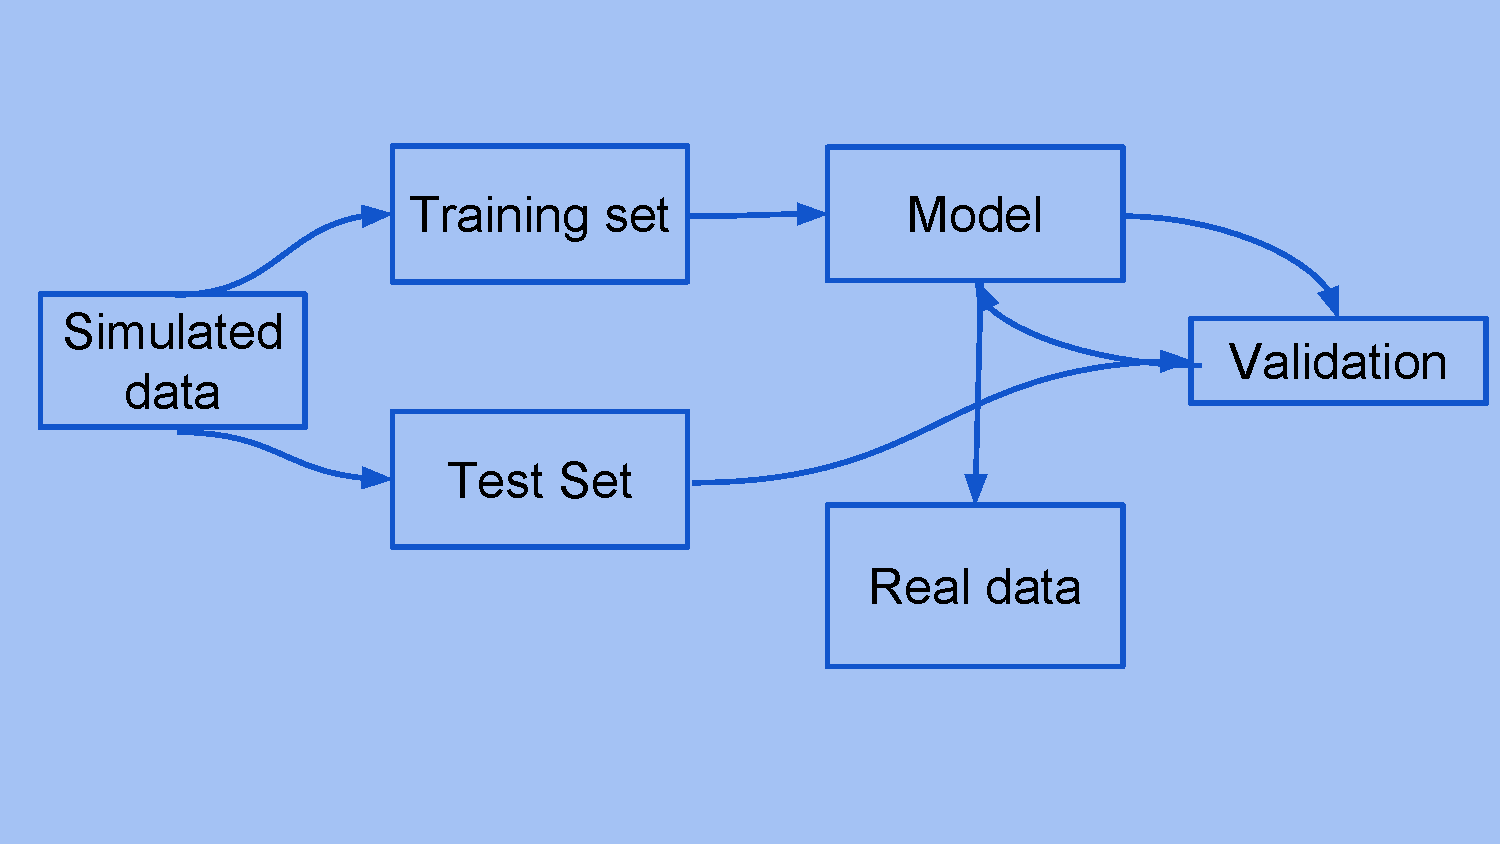
\includegraphics[scale=0.45]{./aprendizaje_supervisado.pdf}
  \end{center}
}

%\frame{
% \frametitle{Simple Example:ANNz}
%  ANNz: Estimating photometric redshift using artificial neural network. Collister \& Lahav 2003 (0311058)
%  \begin{center}
%   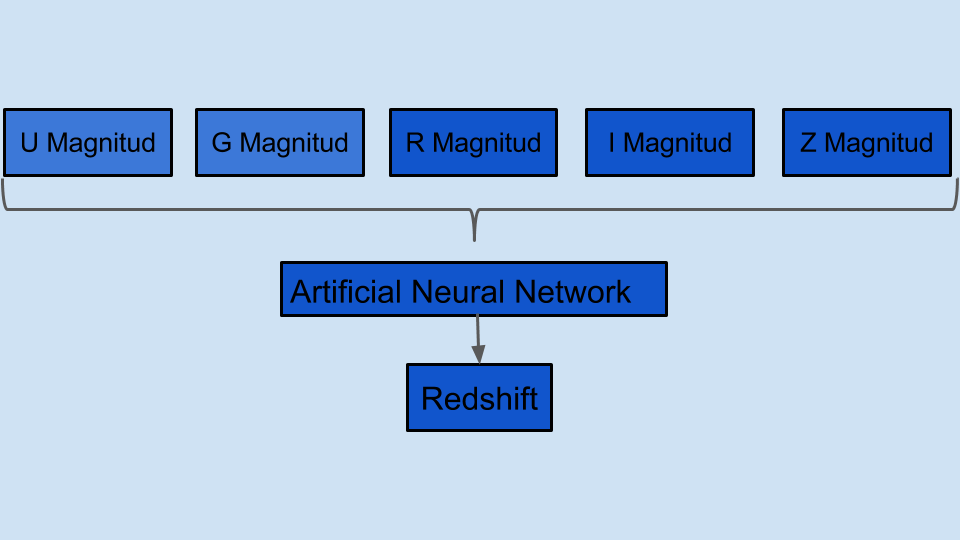
\includegraphics[scale=0.3]{./annz1.png}
%  \end{center}
%}
%\frame{
%  \begin{center}
%   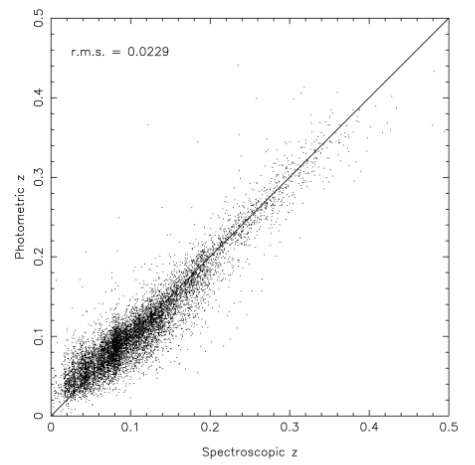
\includegraphics[scale=0.45]{./annz.png}
%  \end{center}
%}

\section{Measuring the Cosmological Parameters.}
\frame{
\tableofcontents[ 
    currentsection, 
    sectionstyle=show/hide, 
    sectionstyle=show/shaded, 
    ] 
}

%\subsection{What are the cosmological parameters?}
\frame{\frametitle{The Standard model.}
  
  Homogeneous and isotropic Universe $\rightarrow$ FRW metric

  $ds^{2}=dt^{2}-a^{2}(t)[\frac{dr^{2}}{1-kr^{2}}+r^{2}(d \theta^{2}+sin^{2} \theta d \phi^{2})] $

  $(\frac{H}{H_{0}})^{2}=\Omega_{rad}a^{-4}+\Omega_{m}a^{-3}+\Omega_{\Lambda}-Kc^{2}a^{-2}$

  \begin{center}
 %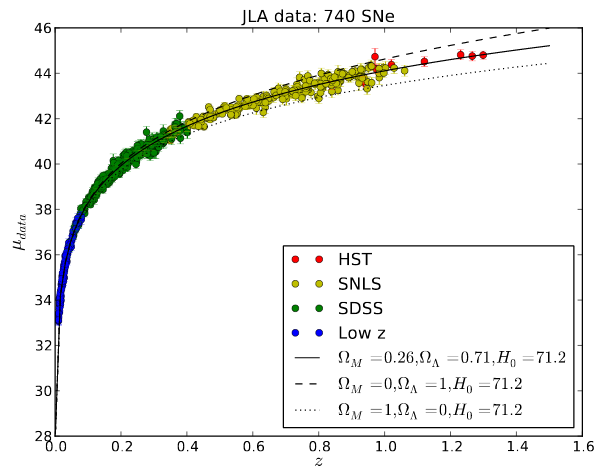
\includegraphics[scale=0.26]{./supernovas.png}
  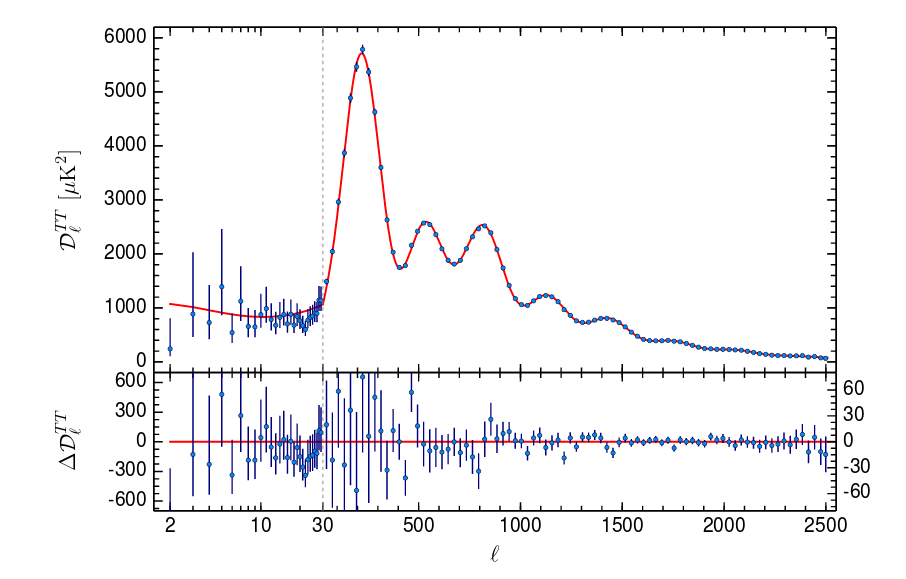
\includegraphics[scale=0.22]{./planck.png}
 % supernovas.png: 0x0 pixel, 300dpi, 0.00x0.00 cm, bb=
  \end{center}
Planck Collaboration 2015 (1502.01589)
} 

\subsection{The training sample.}
\frame{
\frametitle{The training sample.}
CAMB: Code for Anisotropies in the Cosmic Background 
\begin{center}
 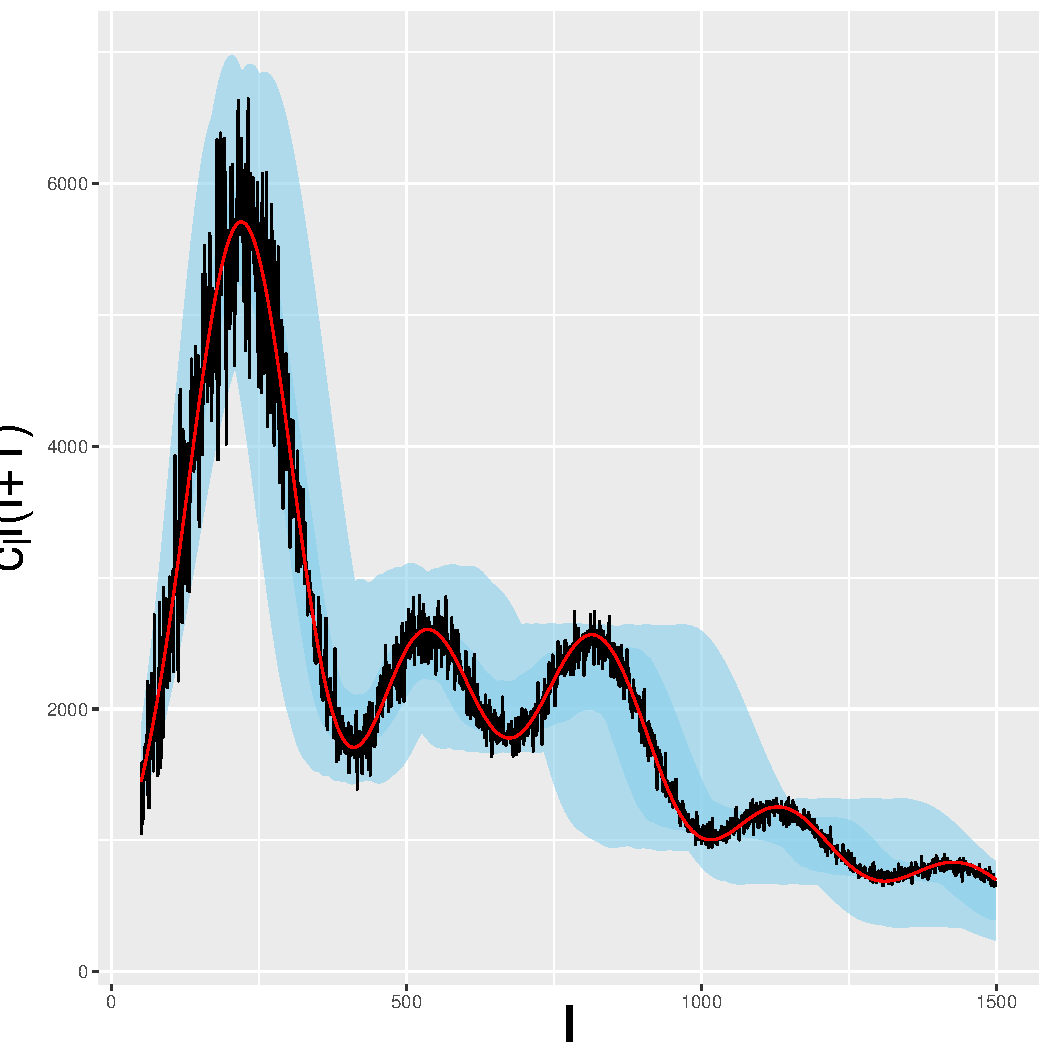
\includegraphics[scale=0.3]{./fig1_nueva.pdf}
  %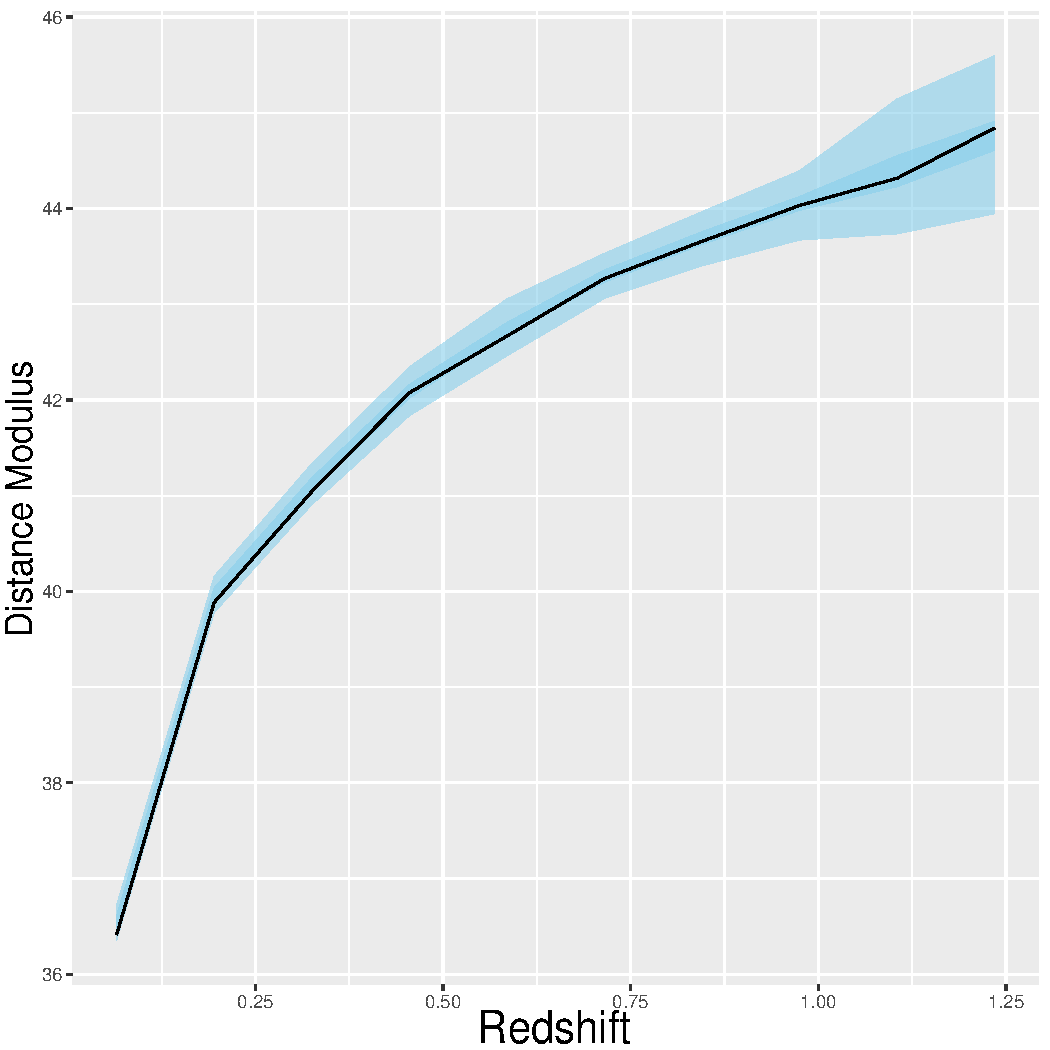
\includegraphics[scale=0.3]{./fig2_nueva.pdf}
 % fig1_nueva.pdf: 0x0 pixel, 300dpi, 0.00x0.00 cm, bb=
\end{center}

}

%\subsection{Studying different Machine Learning algorithms.}
\frame{\frametitle{Studying different Machine Learning algorithms.}
\begin{center}
 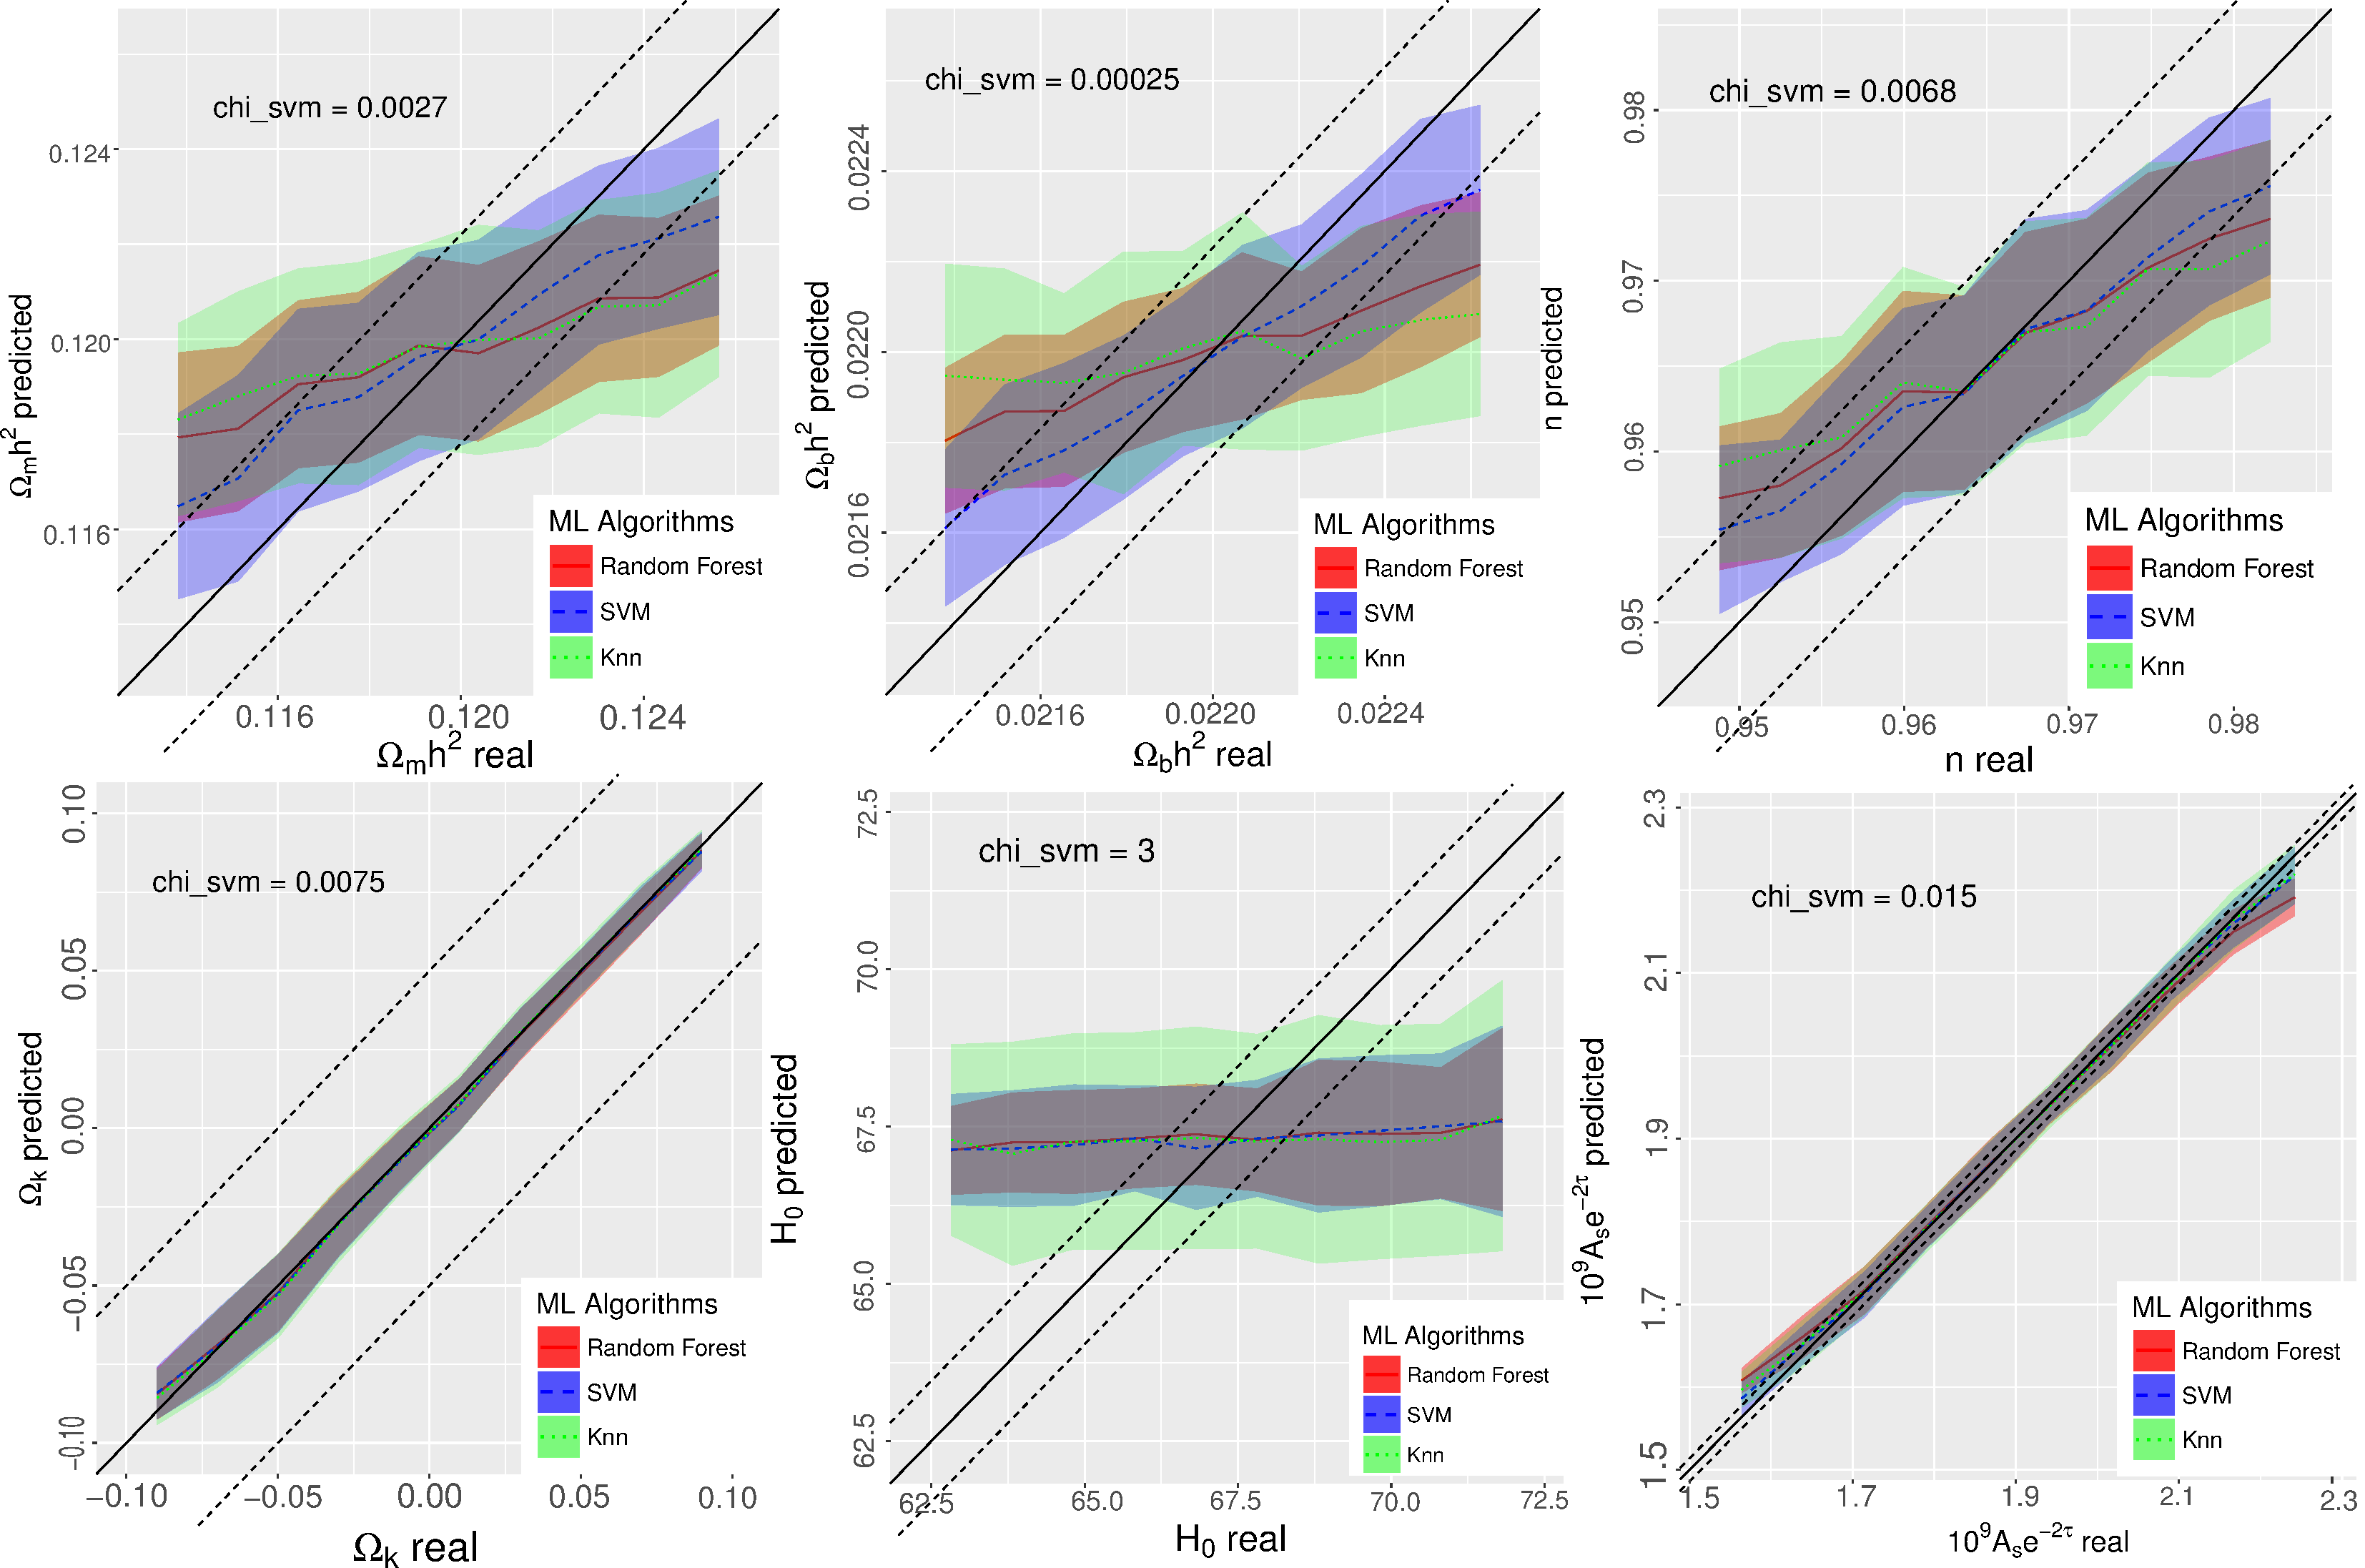
\includegraphics[scale=0.18]{./predicciones.pdf}
 % fig3_paper.pdf: 0x0 pixel, 300dpi, 0.00x0.00 cm, bb= width=32,height=23
\end{center}

}


\subsection{Applications.}

\frame{
\frametitle{Measuring the cosmological parameters angular distributions. }
\begin{figure}[ht!]
 \centering
 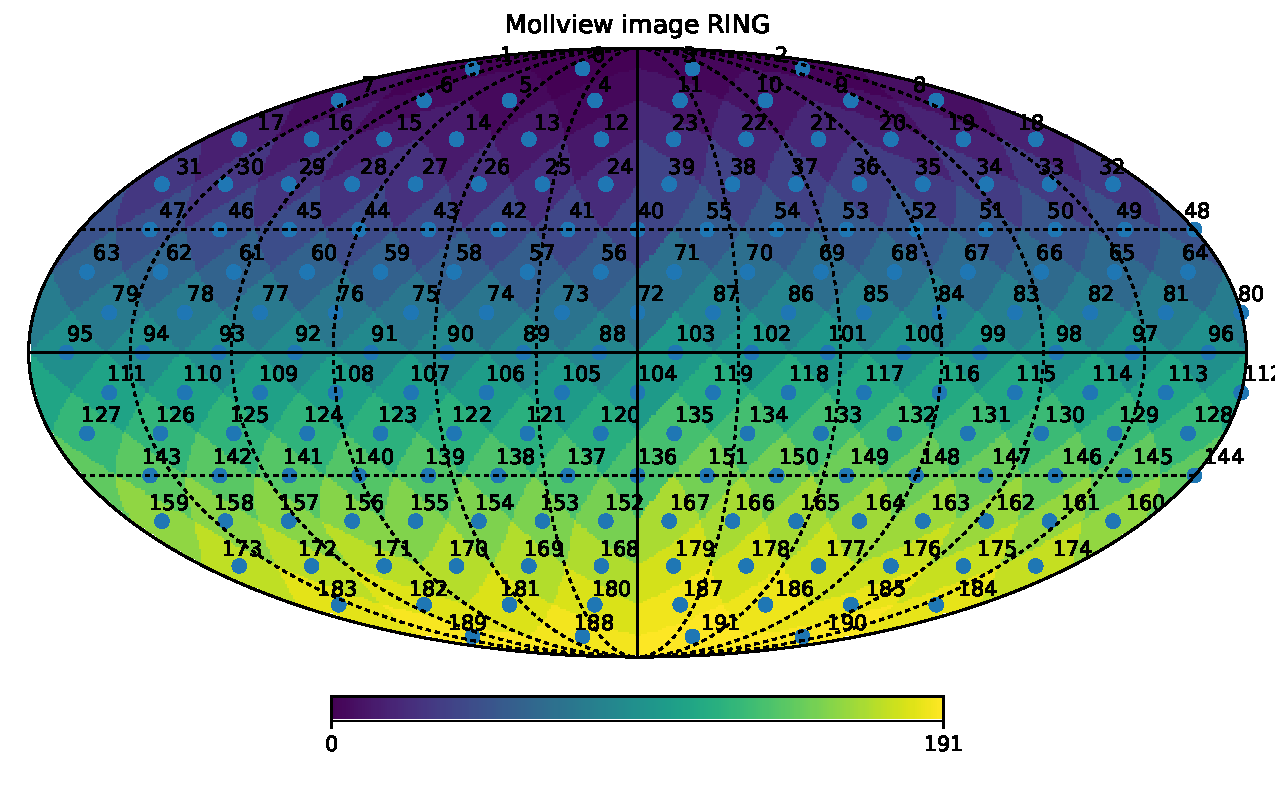
\includegraphics[scale=0.5,keepaspectratio=true]{./map-nside4.pdf}
 % map-nside4.pdf: 0x0 pixel, 300dpi, 0.00x0.00 cm, bb=
\end{figure}

}

\frame{
\frametitle{Measuring the cosmological parameters angular distributions. }

\begin{figure}[l]
 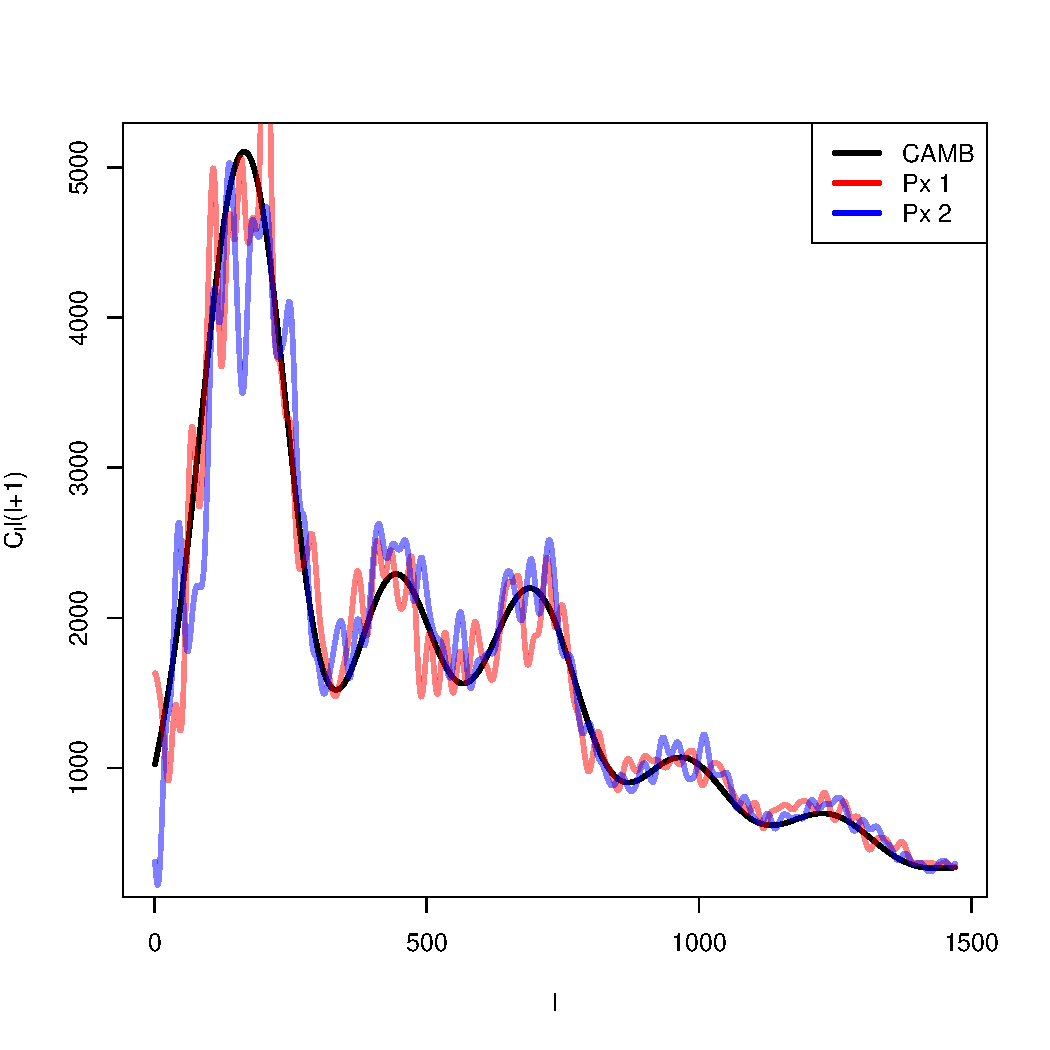
\includegraphics[scale=0.4,keepaspectratio=true]{./pixelado.pdf}
\end{figure}
}

\frame{
\frametitle{Denoising Autoencoders}

\begin{figure}[ht!]
 \centering
 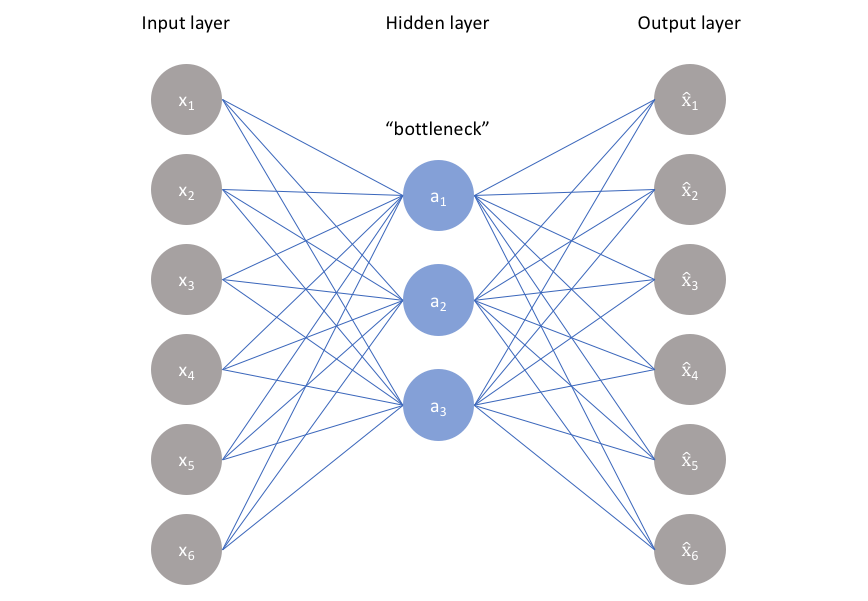
\includegraphics[scale=0.3,keepaspectratio=true]{./autoencoder.png}
\end{figure}

}

\frame{
\frametitle{Denoising Autoencoders}

\begin{figure}[ht!]
 \centering
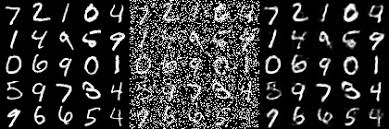
\includegraphics[scale=0.7,keepaspectratio=true]{./daes.jpeg}
\end{figure}

}

\frame{
\frametitle{Denoising Autoencoders}

\begin{figure}[ht!]
 \centering
 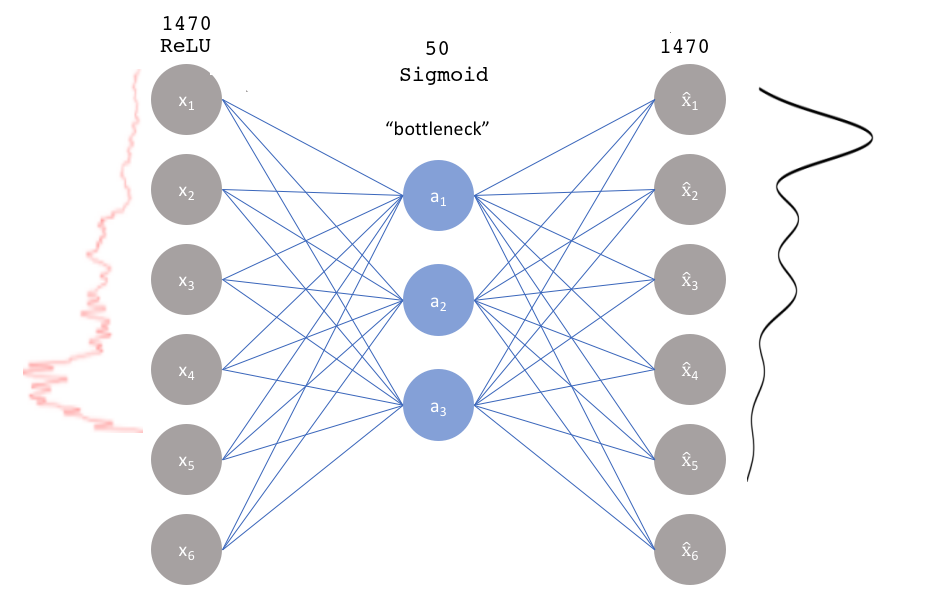
\includegraphics[scale=0.5,keepaspectratio=true]{./autoencoder2.png}
\end{figure}

}
%\frame{
%\begin{figure}[l]
% 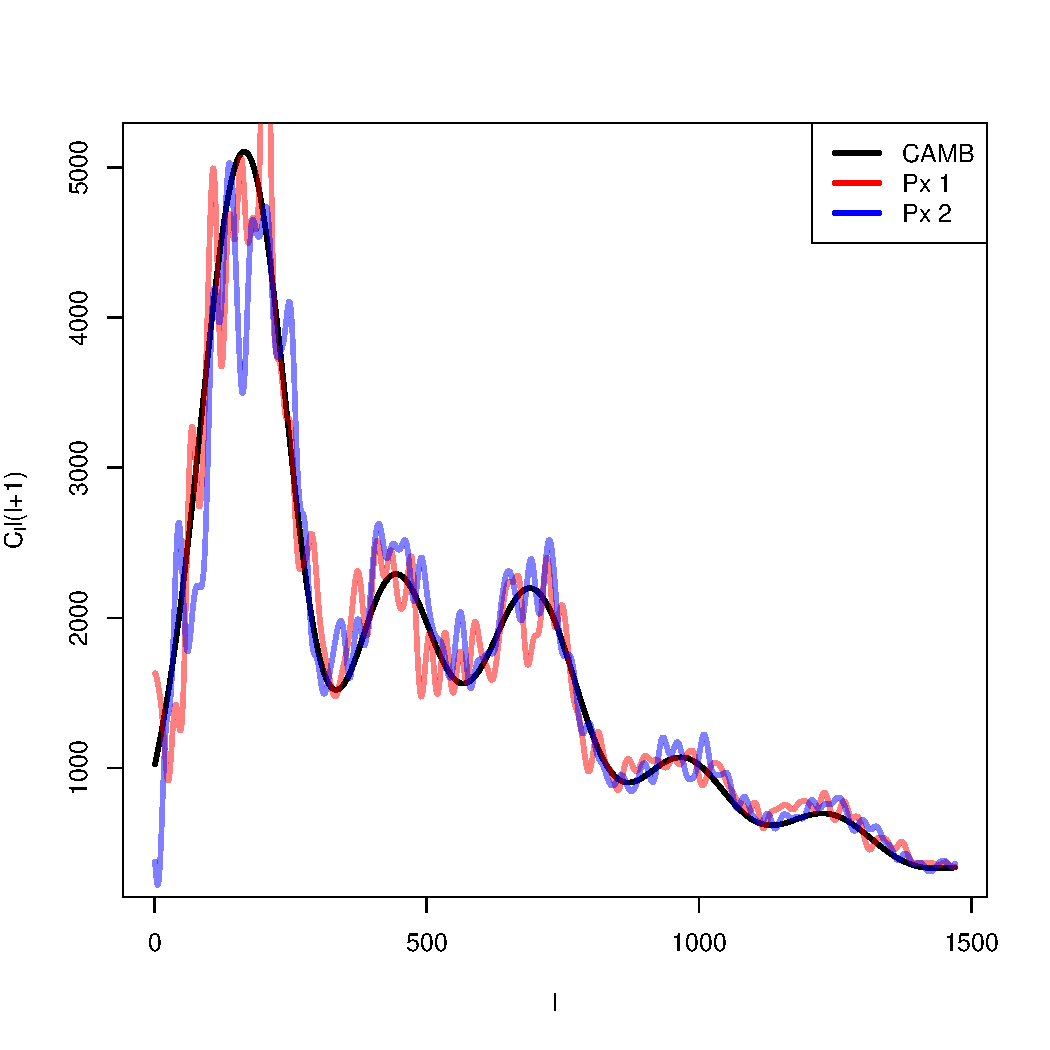
\includegraphics[width=5cm,height=5cm]{./pixelado.pdf}
 % pixelado.pdf: 0x0 pixel, 300dpi, 0.00x0.00 cm, bb=
% 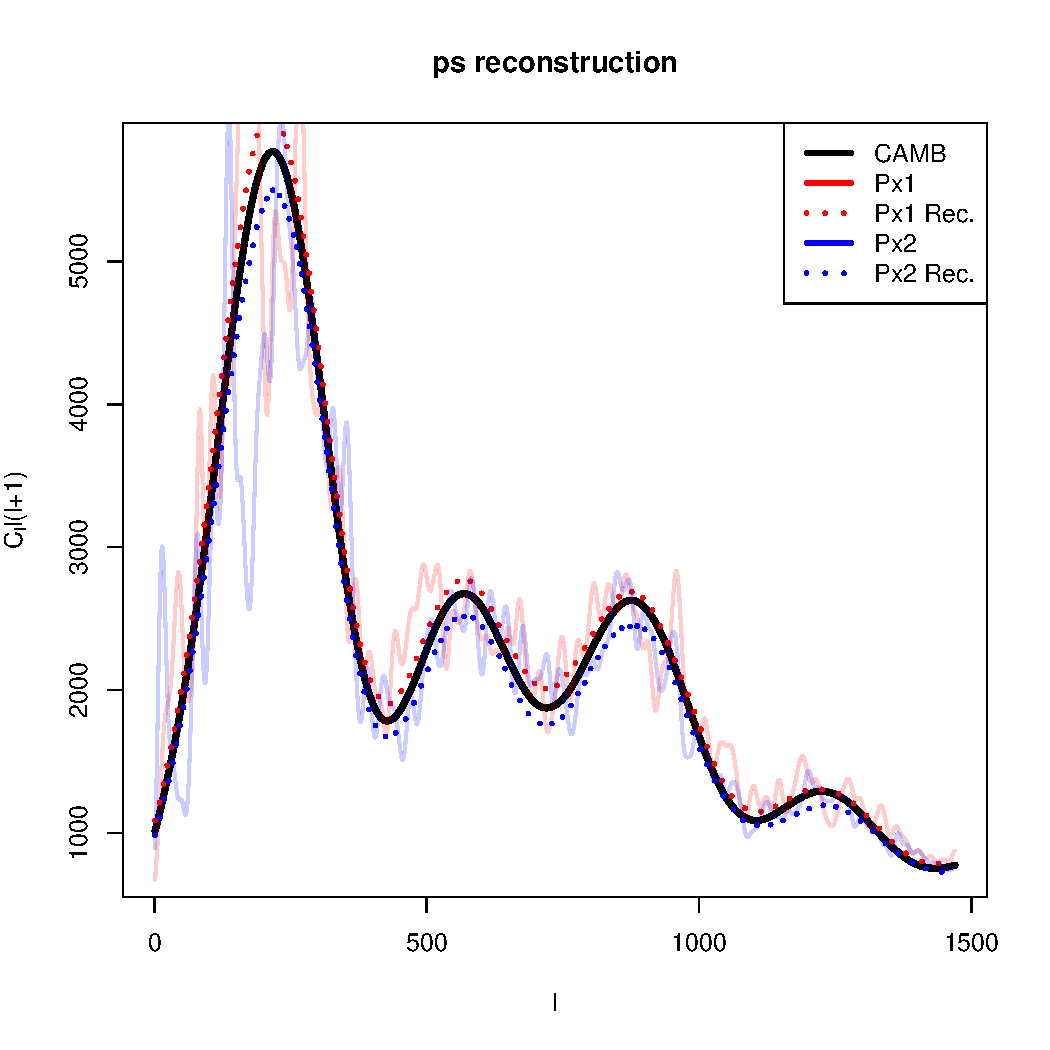
\includegraphics[width=5cm,height=5cm]{./pixelado_reconstruction.pdf}
 % pixelado_reconstruction.pdf: 0x0 pixel, 300dpi, 0.00x0.00 cm, bb=
%\end{figure}
%}

\frame{
\begin{figure}[ht!]
 \centering
 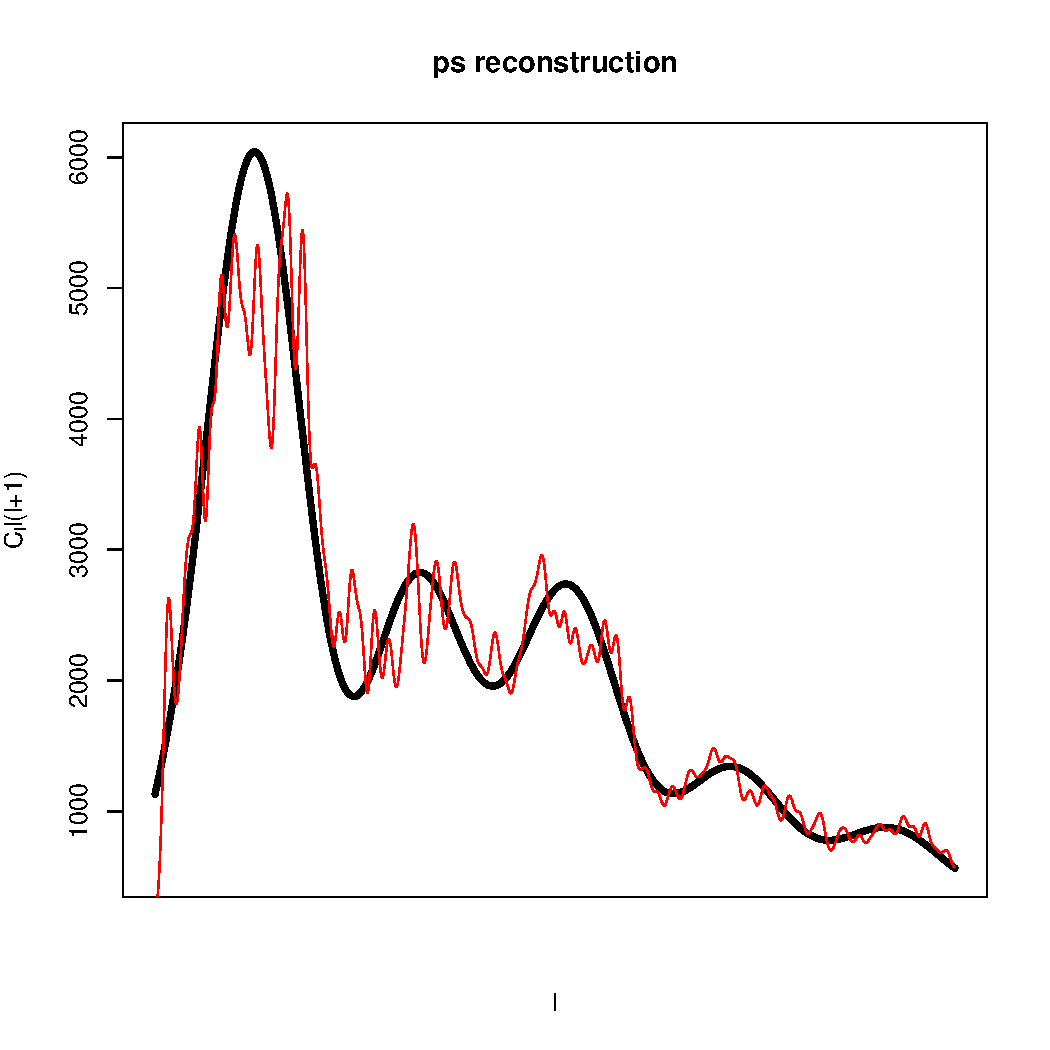
\includegraphics[scale=0.5,keepaspectratio=true]{./pixel1.pdf}
 % pixel1.pdf: 0x0 pixel, 300dpi, 0.00x0.00 cm, bb=
\end{figure}
}
\frame{
\begin{figure}[ht!]
 \centering
 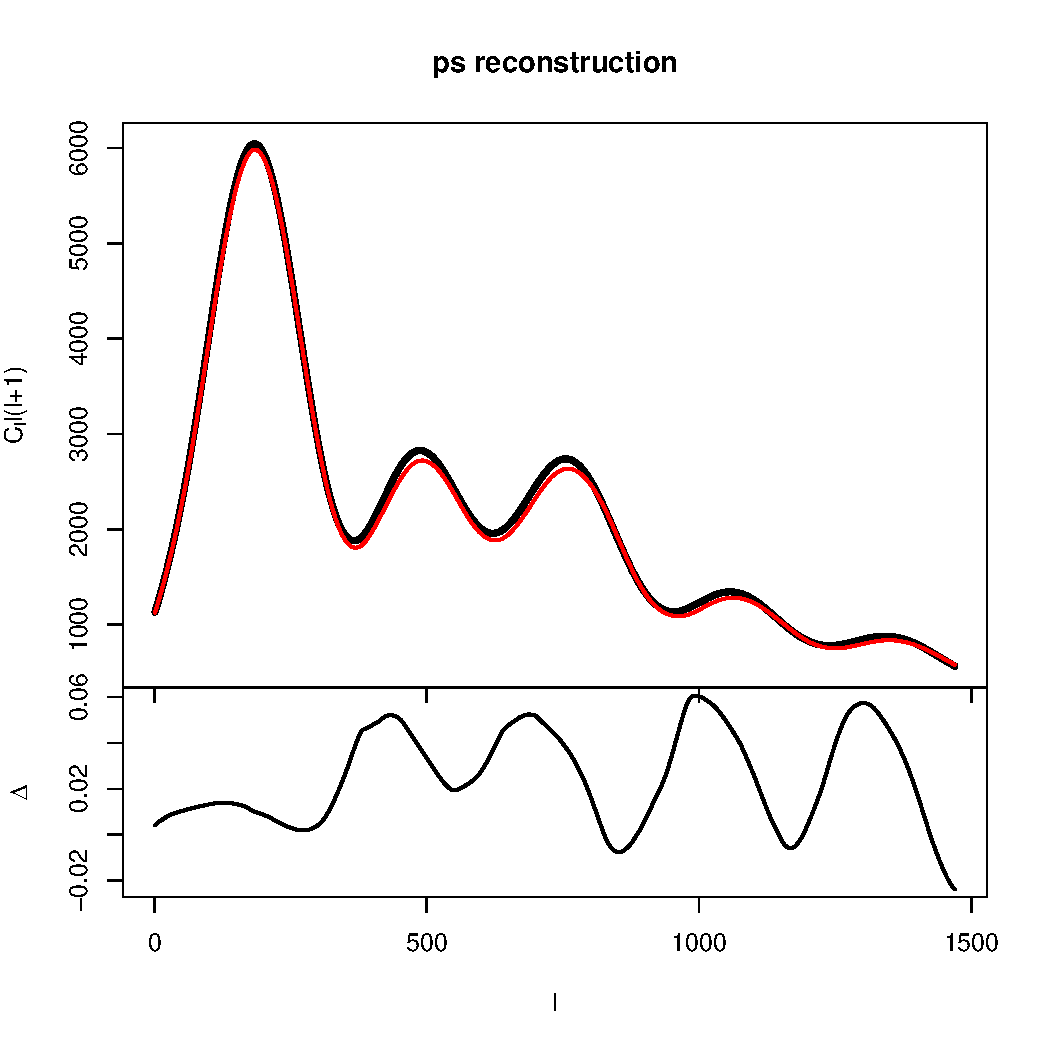
\includegraphics[scale=0.5,keepaspectratio=true]{./pixel1_reconstruction.pdf}
 % pixel1.pdf: 0x0 pixel, 300dpi, 0.00x0.00 cm, bb=
\end{figure}
}
\frame{
\begin{figure}[ht!]
 \centering
 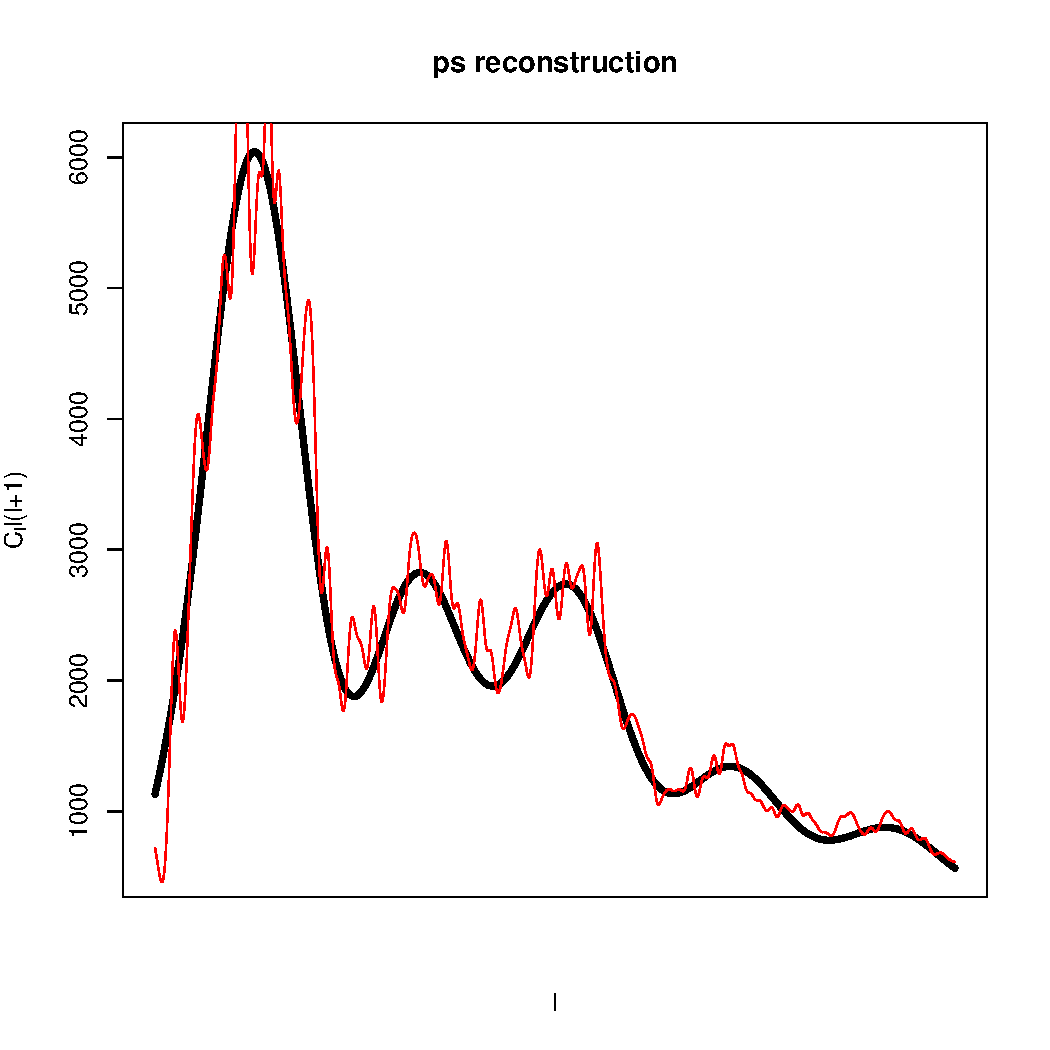
\includegraphics[scale=0.5,keepaspectratio=true]{./pixel2.pdf}
 % pixel1.pdf: 0x0 pixel, 300dpi, 0.00x0.00 cm, bb=
\end{figure}
}
\frame{
\begin{figure}[ht!]
 \centering
 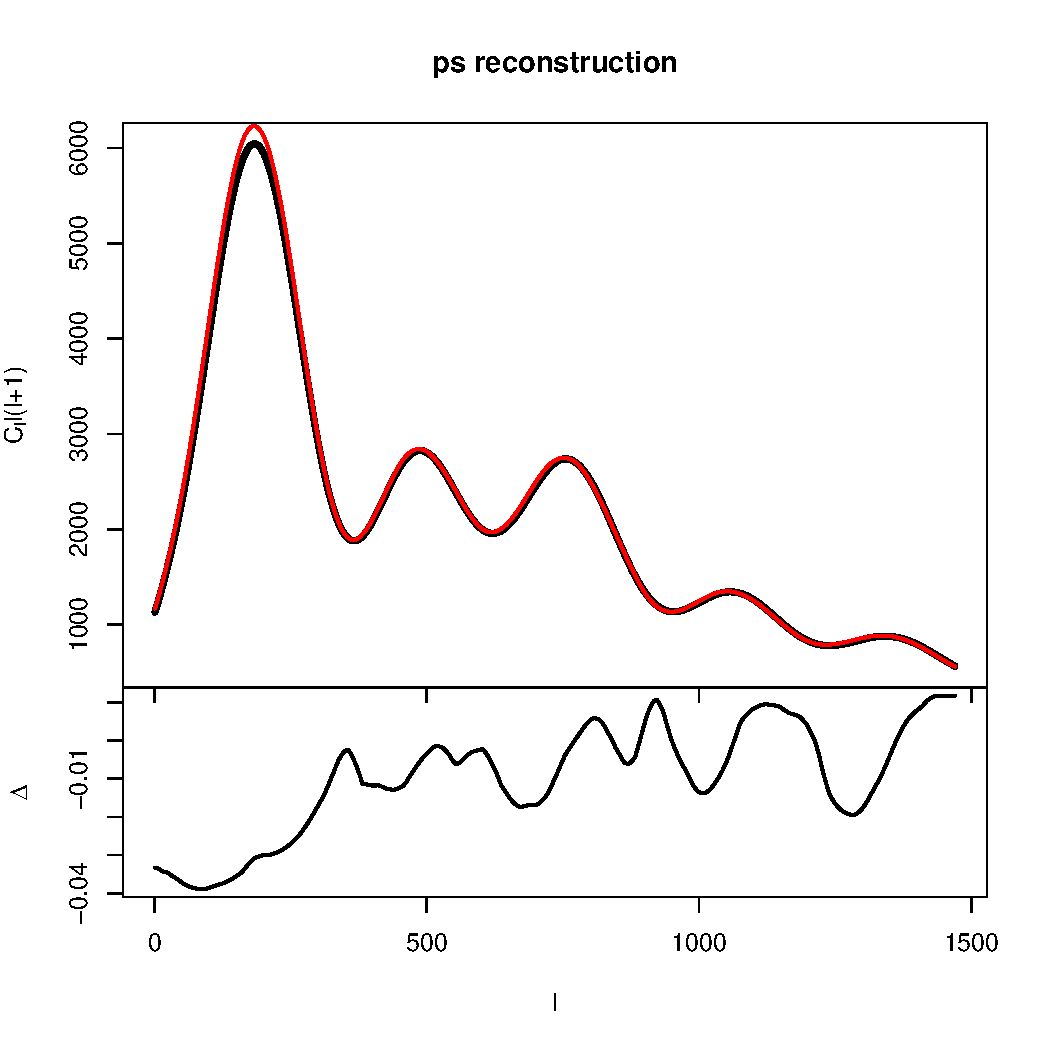
\includegraphics[scale=0.5,keepaspectratio=true]{./pixel2_reconstruction.pdf}
 % pixel1.pdf: 0x0 pixel, 300dpi, 0.00x0.00 cm, bb=
\end{figure}
}
\frame{
\frametitle{Measuring the cosmological parameters angular distributions. }

$\chi = \frac{\sum_{i=1}^{npix} |C_{l, real}-C_{l, rec}|}{npix}$

\begin{figure}[]
 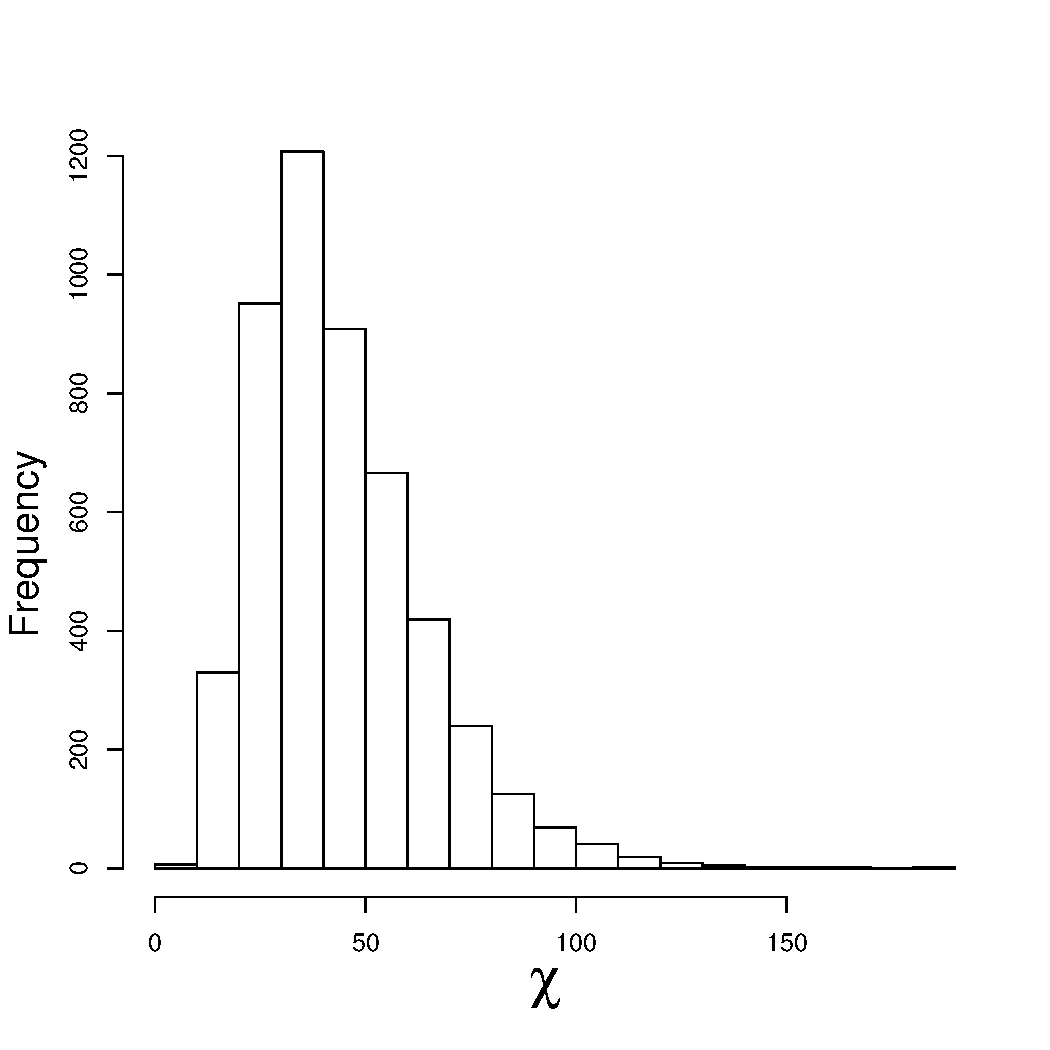
\includegraphics[scale=0.35,keepaspectratio=true]{./chi_DAEs.pdf}
 % chi_DAEs.pdf: 0x0 pixel, 300dpi, 0.00x0.00 cm, bb=
\end{figure}
}

\frame{ 
\begin{figure}[ht!]
 \centering
 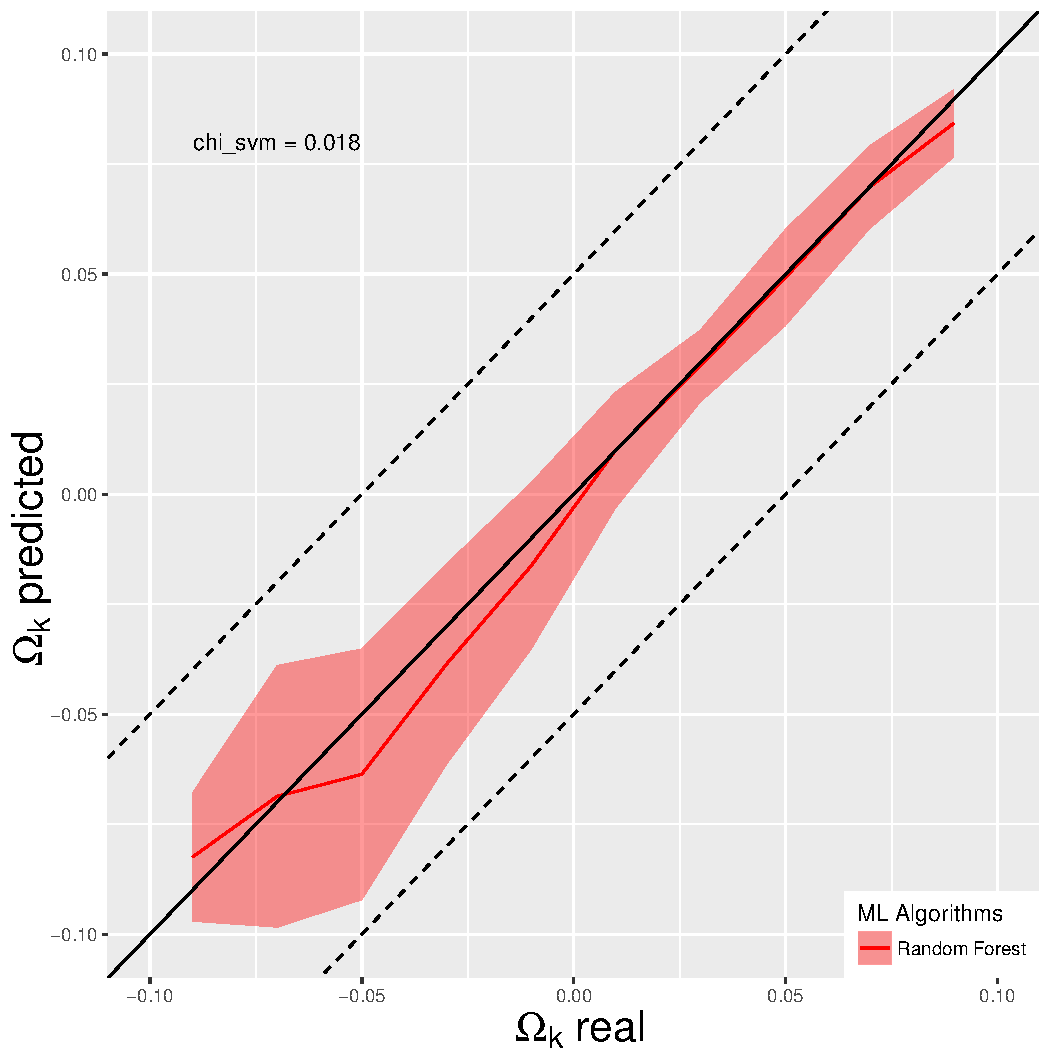
\includegraphics[scale=0.47,keepaspectratio=true]{./omk_pred_pixels_dae.pdf}
 % 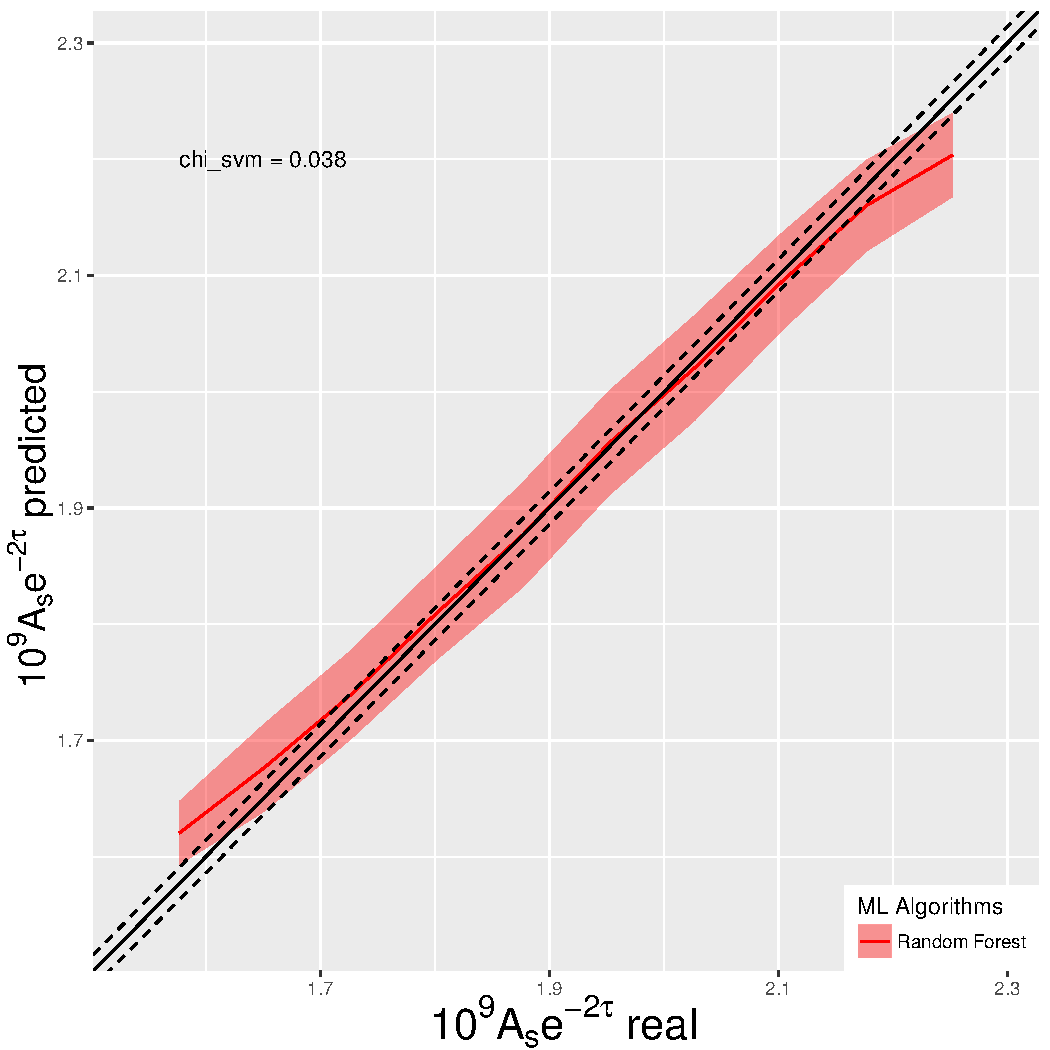
\includegraphics[scale=0.27,keepaspectratio=true]{./at_pred_pixels_dae.pdf}
 % omk_pred_pixels_dae.pdf: 0x0 pixel, 300dpi, 0.00x0.00 cm, bb=
\end{figure}
}

\frame{
\begin{center}
 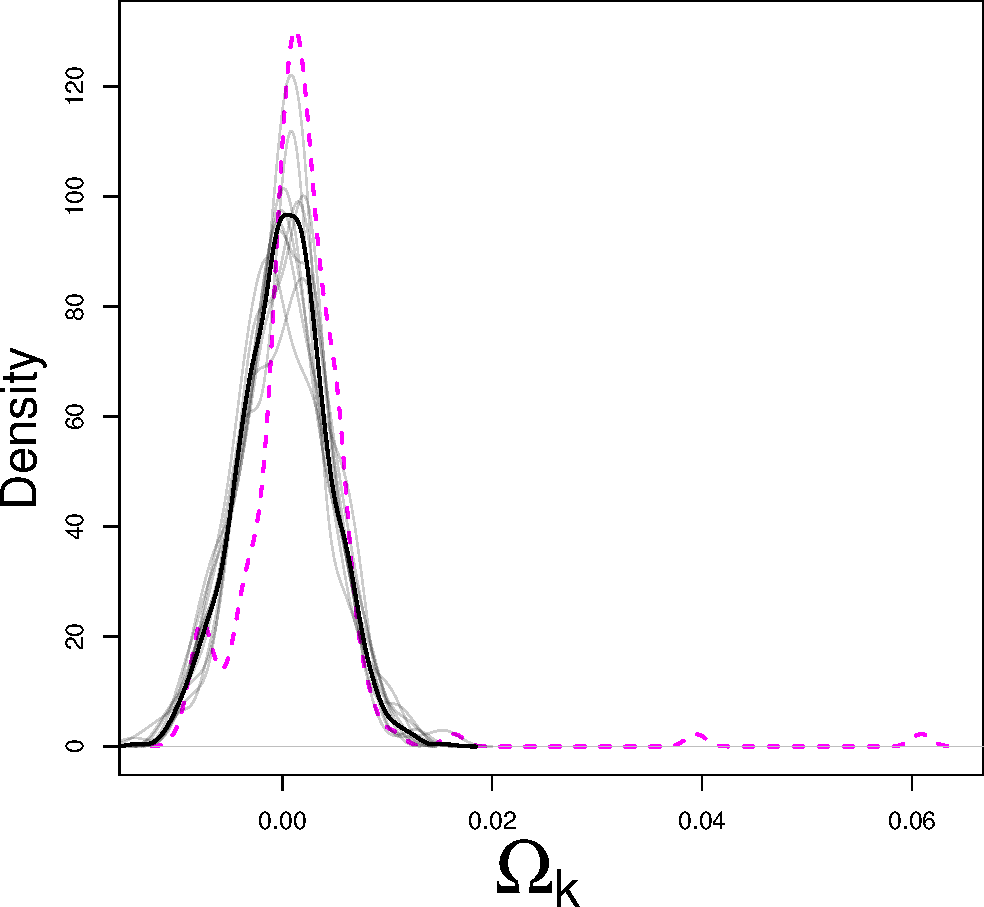
\includegraphics[scale=0.5,keepaspectratio=true]{./omk_predictions.pdf}
 % omk_predictions.pdf: 0x0 pixel, 300dpi, 0.00x0.00 cm, bb
 % fig7_paper.pdf: 0x0 pixel, 300dpi, 0.00x0.00 cm, bb=
\end{center}
}


\section{Final Remarks.}
\frame{
\tableofcontents[ 
    currentsection, 
    sectionstyle=show/hide, 
    sectionstyle=show/shaded, 
    ] 
}
\frame{
\frametitle{Final Remarks}
\begin{small}
 

\begin{itemize}
 \item We developed a machine learning technique that estimate the cosmological parameters in a more efficient way withouth losing precision.
 \item This technique can be easily extended to use more cosmological information as features (BAO, correlation function, SZ emission, etc.).
 %\item We do not found statistically significant departures from what is expected in an homogeneous and isotropic universe, with the possible
 %exception of a bi-modal $H_{0}$ distribution.
 \item As a first application we are studying the angular distribution of the cosmological parameters.
 \item We do not found any significant curvature departure from what is expected in an homogeneous and isotropic univese, with the exception of 
 some pixels that are in the galactic plane.
 \item We will extend the parameters space and add polarization information in a forthcoming work.
 \item We will analyze the correlations between the angular distribution of the cosmological parameters and the large scale structure (voids, filaments, etc.) 
\end{itemize}
\end{small}

}
\frame{
 \begin{center}
 
\includegraphics[scale=0.45]{./thankyou.png}
 % comparaciones.pdf: 0x0 pixel, 300dpi, 0.00x0.00 cm, bb=
\end{center}

}


\frame{
Changing the minimum mutipole.

\begin{center}
 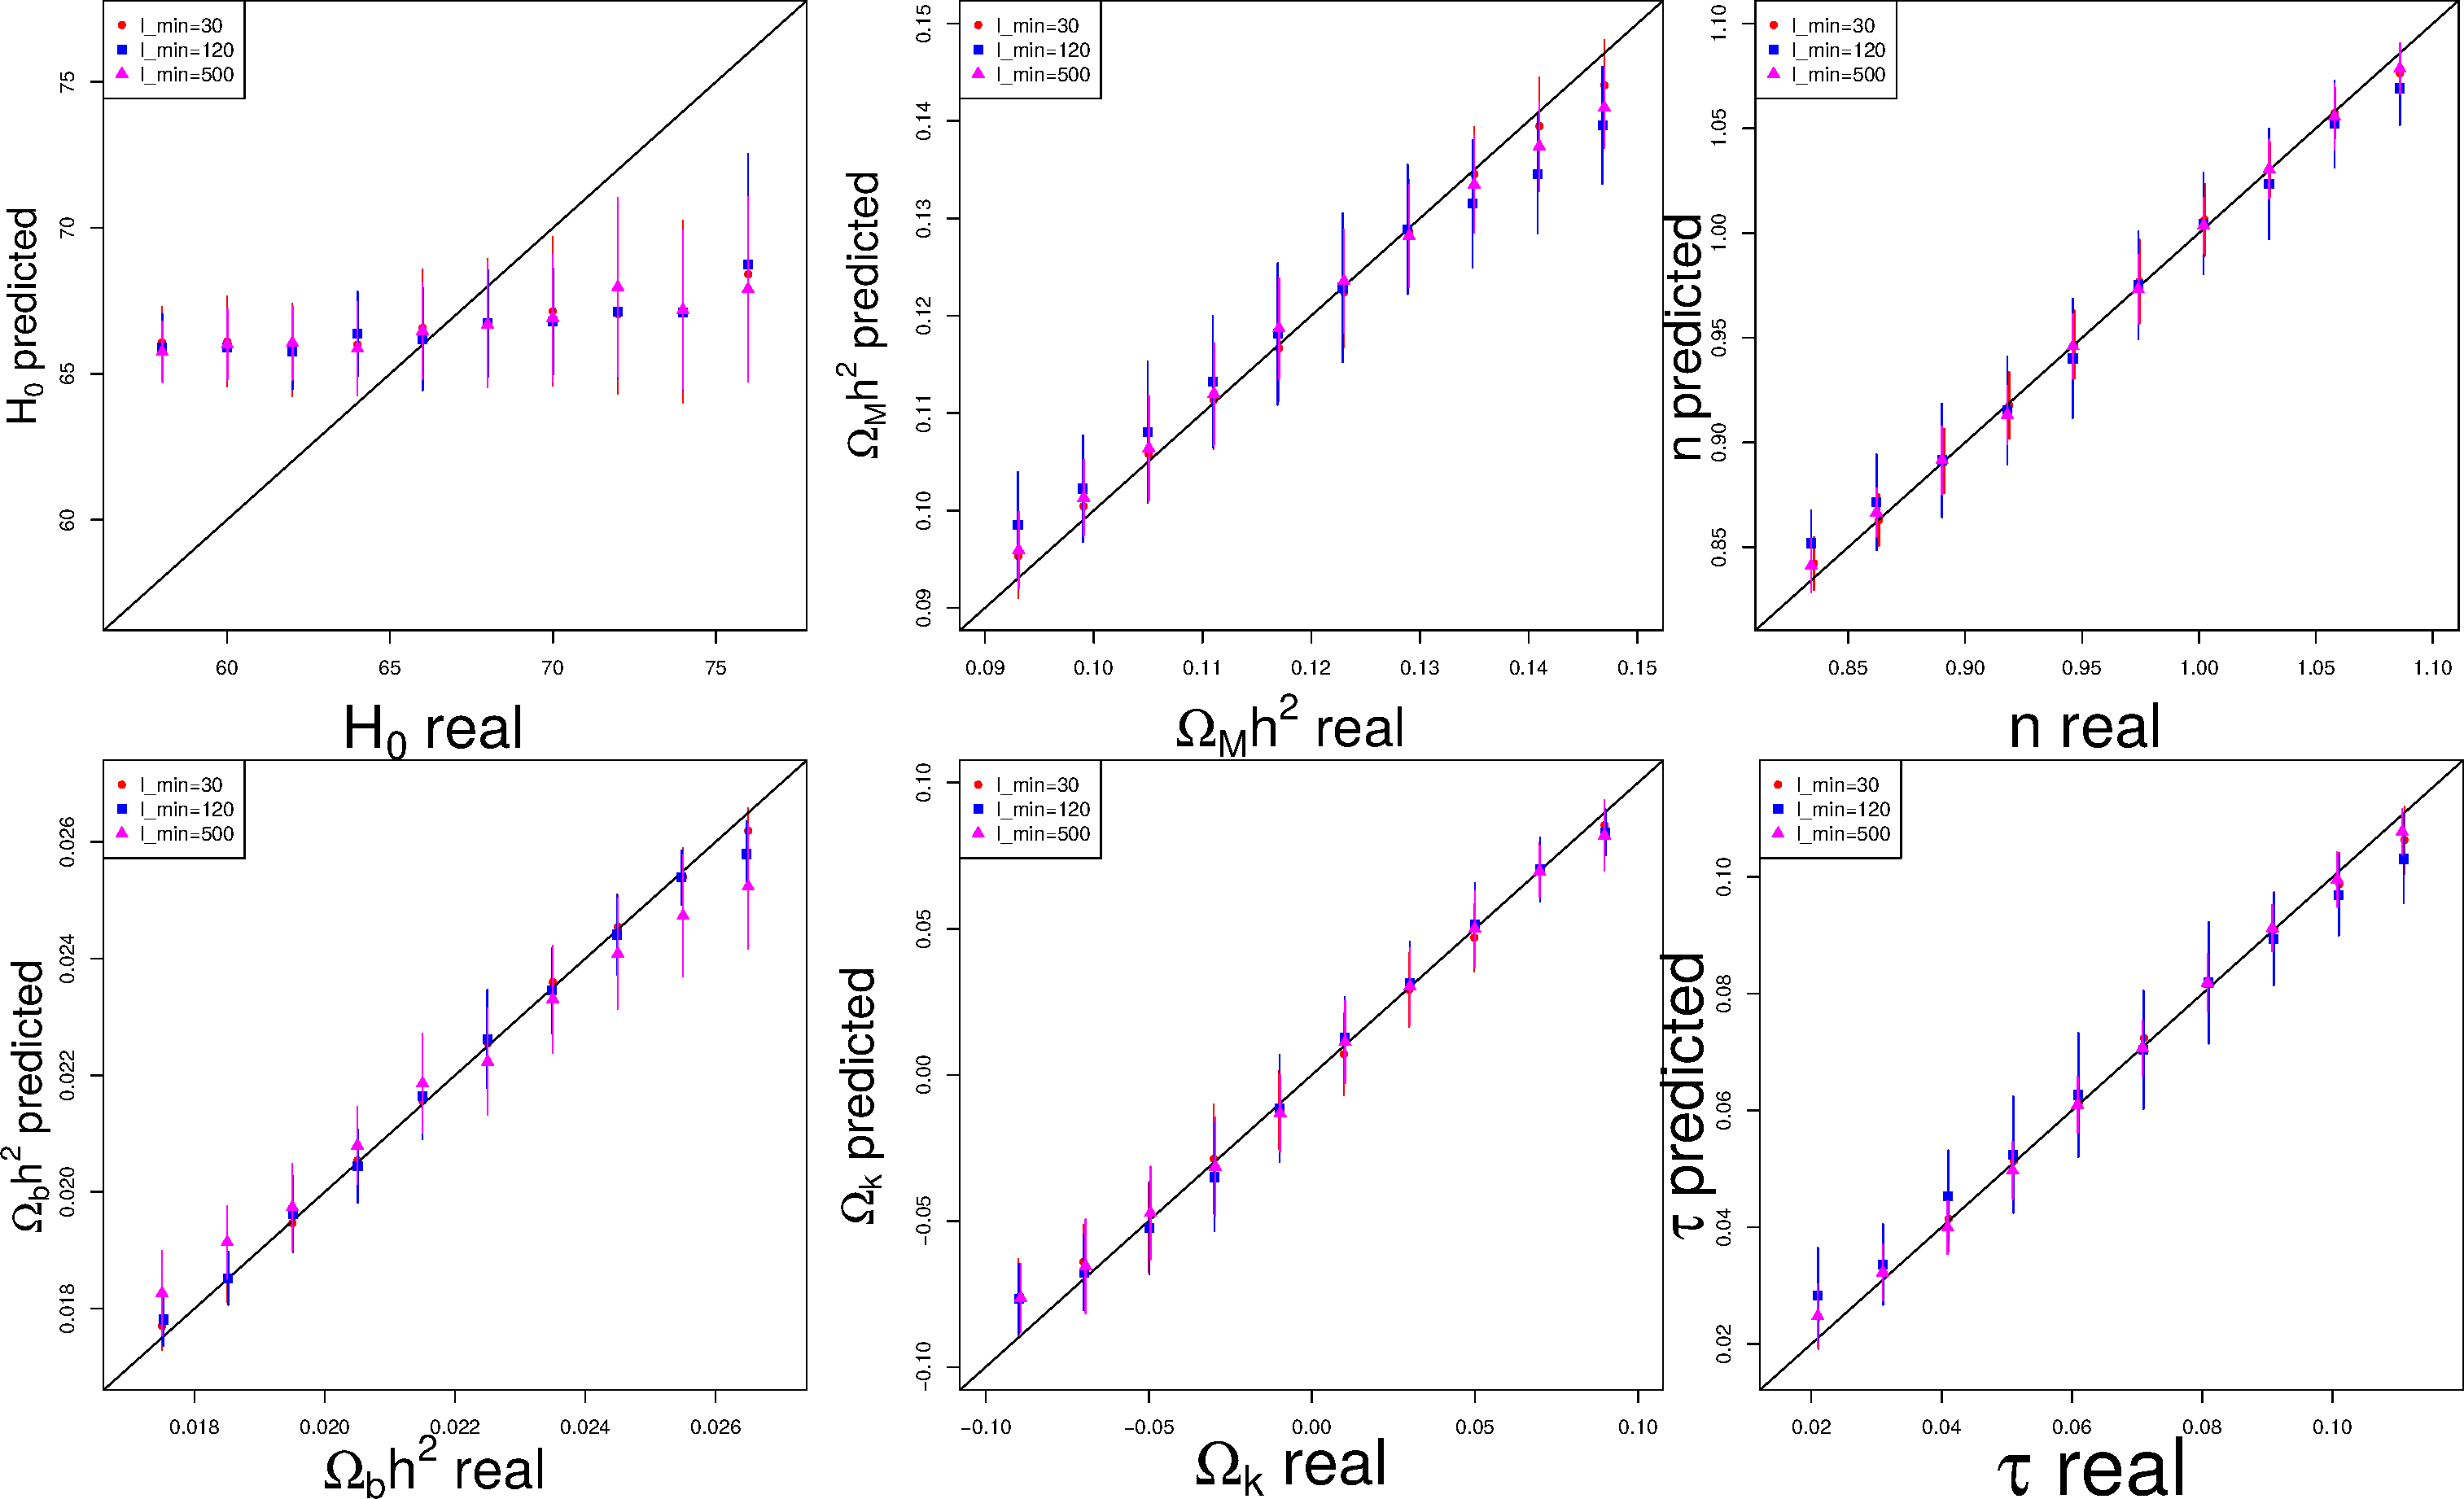
\includegraphics[scale=0.2]{./lvar.pdf}
 % lvar.pdf: 0x0 pixel, 300dpi, 0.00x0.00 cm, bb=
\end{center}

}

\end{document}

